\documentclass[11pt, a4paper]{article}

\usepackage[top=1 in, bottom = 1 in, left = 1 in, right = 1 in ]{geometry}

\usepackage{amsmath, amssymb, amsfonts}
\usepackage{enumerate}
\usepackage{multirow}
\usepackage{hhline}
\usepackage{array}
\usepackage{longtable}
\usepackage{graphicx}

\title{\textbf{QUESTIONS}}

\author{}
\date{}

\begin{document}

\maketitle

\begin{enumerate}

%01

	\item The average number of days survived by mice inoculated with 5 strains of typhoid organisms along with their standard deviation and number of mice involved in each experiment is given below. On the basis of these data, what would be your conclusions regarding the strains of typhoid organisms ?
	
	\begin{table}[h]
	\def\arraystretch{1.5}
	
	\begin{center}
	\begin{tabular}{|>{\centering}m{4 cm}|>{\centering}m{1.5 cm}>{\centering}m{1.5 cm}>{\centering}m{1.5 cm}>{\centering}m{1.5 cm}>{\centering\arraybackslash}m{1.5 cm}|}
	
	\hline
	
	Strains of typhoid & A & B & C & D & E \\
	
	\hline
	
	No. of mice, $n_i$ & 10 & 6 & 8 & 11 & 5 \\
	
	Average, $\overline{y_i}$ & 10.9 & 13.5 & 11.5 & 11.2 & 15.4 \\
	
	Standard deviation, $s_i$ & 12.72 & 5.96 & 3.24 & 5.65 & 3.64 \\
	
	\hline
	\end{tabular}
	\end{center}
	\end{table}
	
	
	
	
	
\vspace{40pt}	
	





%02
	\item 
	\begin{enumerate}[(a)]
		\item A manufacturing company has purchased three new machines of different makes and wishes to determine whether one of them is faster than the others in producing a certain output. Five-hourly production figures are observed at random from each machine and the results are as follows.
		
		\begin{table}[h]
		\def\arraystretch{1.5}
		
		\begin{center}
		\begin{tabular}{|>{\centering}m{3 cm}|>{\centering}m{1.5 cm}|>{\centering}m{1.5 cm}|>{\centering\arraybackslash}m{1.5 cm}|}
		
		\hline
		
		& Machine $A_1$ & Machine $A_2$ & Machine $A_3$ \\
		
		\hline
		
		& 25 & 31 & 24 \\
		
		& 30 & 39 & 30 \\
		
		Observations & 36 & 38 & 28 \\
		
		& 38 & 42 & 25 \\
		
		& 31 & 35 & 28 \\
		
		\hline
		
		\end{tabular}
		\end{center}
		
		\end{table}
		
		Use analysis of variance technique and determine whether the machines are signifacntly different in their mean speeds. Use $\alpha = 5 \%$.
		
		\item Analyse the above data after shifting the origin to 30. How are the results in Part (a) affected ? Explain.
	
	\end{enumerate}
	
	
	
	
	
	
\newpage
	
	
	
	
%03
	\item The following table gives quality rating of ten service stations by five professional raters.
	
	\begin{table}[h]
	\def\arraystretch{1.5}
	
	\begin{center}
	\begin{tabular}{|c|>{\centering}m{1 cm}>{\centering}m{1 cm}>{\centering}m{1 cm}>{\centering}m{1 cm}>{\centering}m{1 cm}>{\centering}m{1 cm}>{\centering}m{1 cm}>{\centering}m{1 cm}>{\centering}m{1 cm}>{\centering\arraybackslash}m{1 cm}|}
	
	\hline
	
	\multirow{2}{*}{RATER} & \multicolumn{10}{c|}{SERVICE STATION} \\
	
	\hhline{~----------}
	
	& 1 & 2 & 3 & 4 & 5 & 6 & 7 & 8 & 9 & 10 \\
	
	\hline
	
	A & 99 & 70 & 90 & 99 & 65 & 85 & 75 & 70 & 85 & 92 \\
	
	B & 96 & 65 & 80 & 95 & 70 & 88 & 70 & 51 & 84 & 91 \\
	
	C & 95 & 60 & 48 & 87 & 48 & 75 & 71 & 93 & 80 & 93 \\
	
	D & 98 & 65 & 70 & 95 & 67 & 82 & 73 & 94 & 86 & 80 \\
	
	E & 97 & 65 & 62 & 99 & 60 & 80 & 76 & 92 & 90 & 89 \\
	
	\hline
	
	\end{tabular}
	\end{center}
	
	\end{table}
	
	Analyse the data and discuss whether there is any significant difference between raters or between service stations.
	
	
	
	
\vspace{15pt}	
	
	
	
	
%04
	\item The following data shows the birth-weights of babies born, classified according to the age of mother and order of gravida, there being three observations per cell :
	
	\begin{table}[h]
	\def\arraystretch{1.5}
	
	\begin{center}
	\begin{tabular}{|c|c|c|c|c|c|}
	
	\hline
	
	\multirow{2}{*}{Order of gravida} & \multicolumn{5}{c|}{Age-group of mother} \\
	
	\hhline{~-----}
	
	& 15-20 & 20-25 & 25-30 & 30-35 & 35 and over \\
	
	\hline
	
	1 & 5.1, 5.0, 4.8 & 5.0, 5.1, 5.3 & 5.1, 5.1, 4.9 & 4.9, 4.9, 5.0 & 5.0, 5.0, 5.0 \\
	
	2 & 5.2, 5.2, 5.4 & 5.3, 5.3, 5.5 & 5.3, 5.2, 5.2 & 5.2, 5.0, 5.5 & 5.1, 5.3, 5.0 \\
	
	3 & 5.8, 5.7, 5.9 & 6.0, 5.9, 6.2 & 5.8, 5.9, 5.9 & 5.8, 5.5, 5.5 & 5.9, 5.4, 5.5 \\
	
	4 & 6.0, 6.0, 5.9 & 6.2, 6.5, 6.0 & 6.0, 6.1, 6.0 & 6.0, 5.8, 5.5 & 5.8, 5.6, 5.5 \\
	
	5 and over & 6.0, 6.0, 6.0 & 6.0, 6.1, 6.3 & 5.9, 6.0, 5.8 & 5.9, 6.0, 5.5 & 5.5, 6.0, 6.2 \\
	
	\hline
	
	\end{tabular}
	\end{center}
	
	\end{table}
	
	Test whether the age of mother and order of gravida significantly affect the birth-weight.
	
	
	

\vspace{15pt}	
	
	
	
%05
	
	\item An experiment was conducted to determine the effects of different dates of planting and different methods of planting on the yield of sugar-cane. The data below show the yields of sugar-cane (in kg.) for four different dates and three methods of planting.
	
	\begin{table}[h]
	\def\arraystretch{1.5}
	
	\begin{center}
	\begin{tabular}{|c|c|c|c|c|}
	
	\hline
	
	\multirow{2}{*}{Method of Planting} & \multicolumn{4}{c|}{Date of planting} \\
	
	\hhline{~----}
	
	& October & November & February & March \\
	
	\hline
	
	I & 7.10 & 3.69 & 4.70 & 1.90 \\
	
	II & 10.29 & 4.79 & 4.58 & 2.64 \\
	
	III & 8.30 & 3.58 & 4.90 & 1.80 \\
	
	\hline
	
	\end{tabular}
	\end{center}
	
	\end{table}
	
	Carry out an analysis of the above data.
	
	
	
	
	
	
\newpage
	
	
	
	
	
	
%06
	\item The following table provides marks obtained by 20 undergraduate students in Statistics Honours in a college test and in the subsequent University examination. Fit a simple linear regression model to the data.
	
	\begin{table}[h]
	\def\arraystretch{1.5}
	
	\begin{center}
	\begin{tabular}{|>{\centering}m{2cm}|>{\centering}m{5cm}|>{\centering\arraybackslash}m{5cm}|}
	
	\hline
	
	\multirow{2}{*}{Serial No.} & \multicolumn{2}{c|}{Marks Obtained} \\
	
	\hhline{~--}
	
	& in college test & in university examination \\
	
	\hline
	
	1 & 183 & 433 \\
	
	2 & 175 & 393 \\
	
	3 & 134 & 270 \\
	
	4 & 170 & 364 \\
	
	5 & 183 & 399 \\
	
	6 & 167 & 360 \\
	
	7 & 120 & 368 \\
	
	8 & 175 & 358 \\
	
	9 & 126 & 262 \\
	
	10 & 187 & 376 \\
	
	11 & 123 & 326 \\
	
	12 & 121 & 341 \\
	
	13 & 175 & 403 \\
	
	14 & 133 & 326 \\
	
	15 & 144 & 346 \\
	
	16 & 109 & 255 \\
	
	17 & 165 & 362 \\
	
	18 & 114 & 361 \\
	
	19 & 164 & 382 \\
	
	20 & 125 & 319 \\
	
	\hline
	
	
	
	\end{tabular}
	\end{center}		
	\end{table}





\vspace{30pt}




%07
	\item For 20 pairs of fathers and sons, the regression equation of height of son $(y)$ on height of father $(x)$, both measured in $c.m.$, was found to be $$y = 9.29 + 0.932x.$$ Test whether $a$ differs significantly from zero and $b$ differs significantly from unity. For the 20 pairs, $\overline{x} = 168.17$, $\sum \limits_{i = 1}^{20}\left( x_i - \overline{x} \right)^2 = 777.80$ and $\sum \limits_{i = 1}^{20}\left( y_i - \overline{y} \right)^2 = 939.42$.
	
	
	
	
	
	
	
\newpage









%08
	\item The following table shows, for each of 18 cinchona plants, the yield of dry bark (in oz.), the height (in inches) and the girth (in inches) at a height of $6^{\prime \prime}$ from the ground. Fit a multiple linear regression model to the data.
	\begin{table}[!htbp]
	\def\arraystretch{1.5}
	
	\begin{center}
	\begin{tabular}{|>{\centering}m{2cm}|>{\centering}m{4cm}|>{\centering}m{2cm}|>{\centering\arraybackslash}m{4cm}|}
	
	\hline
	
	Plant no. & Yield of dry bark (oz.) & Height (in.) & Girth at a height of $6^{\prime \prime}$ \\
	
	\hline
	
	1 & 19 & 8 & 4 \\
	
	2 & 51 & 15 & 5 \\
	
	3 & 30 & 11 & 3 \\
	
	4 & 42 & 21 & 3 \\
	
	5 & 25 & 7 & 2 \\
	
	6 & 18 & 5 & 1 \\
	
	7 & 44 & 10 & 4 \\
	
	8 & 56 & 13 & 6 \\
	
	9 & 38 & 12 & 3 \\
	
	10 & 32 & 13 & 4 \\
	
	11 & 25 & 5 & 2 \\
	
	12 & 10 & 6 & 3 \\
	
	13 & 20 & 4 & 4 \\
	
	14 & 27 & 8 & 4 \\
	
	15 & 13 & 7 & 3 \\
	
	16 & 49 & 12 & 5 \\
	
	17 & 27 & 6 & 3 \\
	
	18 & 55 & 16 & 7 \\
	
	\hline
	
	\end{tabular}
	\end{center}
	
	\end{table}
	
	
	
	
	
	
\vspace{30pt}	
	
	
	
	
%09
	\item During a crop-cutting survey, a random sample of 16 equal-sized small plots was taken and the green weight $(x)$ and dry weight $(y)$ in kg. of paddy were recorded for each plot. Given that, $$\sum \limits_{i = 1}^{16} x_i = 203.6, \hspace{30pt} \sum \limits_{i = 1}^{16} y_i = 186.6, \hspace{30pt} \sum \limits_{i = 1}^{16}x_i^{2} = 2801.88,$$ $$\sum \limits_{i = 1}^{16}y_i^{2} = 2255.56, \hspace{30pt} \sum \limits_{i = 1}^{16}x_iy_i = 2458.84;$$ obtain the linear regression equation of $y$ on $x$. Hence test whether the regression coefficient differs significantly from zero.
	
	
	
	
	
	
	
	
	
	
	
	
\newpage








%10
	\item Students in a statistics class (taught by one of the authors) claimed that doing the homework had not helped to prepare them for the midterm exam. The exam score $y$ and homework score $x$ (averaged upto the time of midterm) for the 18 students in the class were as follows :
	
	\begin{table}[!htbp]
	\def\arraystretch{1.5}
	
	\begin{center}
	\begin{tabular}{|>{\centering}m{2cm}|>{\centering}m{2cm}||>{\centering}m{2cm}|>{\centering\arraybackslash}m{2cm}|}
	
	\hline
	
	$y$ & $x$ & $y$ & $x$ \\
	
	\hline
	
	95 & 96 & 90 & 93 \\
	
	80 & 77 & 0 & 18 \\
	
	0 & 0 & 95 & 86 \\
	
	0 & 0 & 35 & 0 \\
	
	79 & 78 & 50 & 30 \\
	
	77 & 64 & 72 & 59 \\
	
	72 & 89 & 55 & 77 \\
	
	66 & 47 & 75 & 74 \\
	
	98 & 90 & 66 & 67 \\
	
	\hline
	
	
	\end{tabular}
	\end{center}
	
	\end{table}
	Based on this data, verify the students' claim.
	
	
	
	
	
	
	
	
\vspace{50pt}	


	

%11
	\item The following table gives the birth weights of 8 litters of pigs, the litters being of different sizes. Analyse the data to find if the litter means are different and also determine whether the size of litter is an assignable cause of variation.
	
	\begin{table}[!htbp]
	\def\arraystretch{1.5}
	
	\begin{center}
	\begin{tabular}{|>{\centering}m{2.5cm}|>{\centering}m{1cm}|>{\centering}m{1cm}|>{\centering}m{1cm}|>{\centering}m{1cm}|>{\centering}m{1cm}|>{\centering}m{1cm}|>{\centering}m{1cm}|>{\centering\arraybackslash}m{1cm}|}
	
	
	\hline
	
	Litters & 1 & 2 & 3 & 4 & 5 & 6 & 7 & 8 \\\hline\hline
	
	
	\multirow{10}{*}{Birth weights} & 2.0 & 3.5 & 3.3 & 3.2 & 2.6 & 3.1 & 2.6 & 2.5 \\
	
	\cline{2-9}
	
	& 2.8 & 2.8 & 3.6 & 3.3 & 2.6 & 2.9 & 2.2 & 2.4 \\
	
	\cline{2-9}
	
	& 3.3 & 3.2 & 2.6 & 3.2 & 2.9 & 3.1 & 2.2 & 3.0 \\
	
	\cline{2-9}
	
	& 3.2 & 3.5 & 3.1 & 2.9 & 2.0 & 2.5 & 2.5 & 1.0 \\
	
	\cline{2-9}
	
	& 4.4 & 2.3 & 3.2 & 3.3 & 2.0 & & 1.2 & \\
	
	\cline{2-9}
	
	& 3.6 & 2.4 & 3.3 & 2.5 & 2.1 & & 1.2 & \\
	
	\cline{2-9}
	
	& 1.9 & 2.0 & 2.9 & 2.6 & & & & \\
	
	\cline{2-9}
	
	& 3.3 & 1.6 & 3.4 & 2.8 & & & & \\
	
	\cline{2-9}
	
	& 2.8 & & 3.2 & & & & & \\
	
	\cline{2-9}
	
	& 1.1 & & 3.2 & & & & & \\
	
	\hline
	
	
	
	

	
	\end{tabular}
	\end{center}
	
	\end{table}
	
	
	
	
	
	
	
	
	
	
	
\newpage




	\item Consider the following data :

	\begin{table}[!htbp]
	\def\arraystretch{1.5}
	
	\begin{center}
	\begin{tabular}{|>{\centering}m{1cm}|>{\centering}m{1cm}|m{2.5cm}|}
	
	\hline
	
	$x_1$ & $x_2$ & $y$ \\\hline\hline
	
	17 & 42 & 90 \\
	
	\hline
	
	19 & 45 & 71, 76 \\
	\hline
	
	20 & 29 & 63, 63, 80, 80 \\
	
	\hline
	
	21 & 93 & 80, 64, 82, 66 \\
	
	\hline
	
	25 & 34 & 75, 82 \\
	
	\hline
	
	27 & 98 & 99 \\
	
	\hline
	
	28 & 99 & 73 \\
	
	\hline
	
	30 & 73 & 67, 74 \\
	
	\hline
	
	
	
	\end{tabular}
	\end{center}
	
	\end{table}
	
	Fit the model $y = \beta_0 + \beta_1 x_1 + \beta_2 x_2 + \epsilon$.
	
	
	
	
	
	
	
	
	
	
	
	
	
\vspace{50pt}
	
	
	
	
	
	
	
%13
	\item The following experiment was suggested to test whether subjecting seeds to high temperature and low temperature before planting has any effect on yield. Ten plots were taken and in each 6 seeds were sown at random. Two of the seeds were subjected to high temperatuer (h.t.), two to low temperature (l.t.) and two were subject to controls. The yield of individual plants in gms. are recorded in the following table. Test for the comparison of yields under the two treatmetns and control.
	
	\begin{table}[!htbp]
	\def\arraystretch{1.5}
	
	\begin{center}
	\begin{tabular}{|>{\centering}m{1.5cm}|>{\centering}m{1.5cm}|>{\centering}m{1.5cm}|>{\centering}m{1.5cm}|>{\centering}m{1.5cm}|>{\centering}m{1.5cm}|>{\centering\arraybackslash}m{1.5cm}|}
	
	\hline
	
	\multirow{2}{*}{Plot No.} & \multicolumn{2}{c|}{h.t.} & \multicolumn{2}{c|}{l.t.} & \multicolumn{2}{c|}{Control} \\
	
	\hhline{~------}
	
	& Plant I & Plant II & Plant I & Plant II & Plant I & Plant II \\\hline\hline
	
	1 & 15 & 16 & 20 & 22 & 25 & 24 \\
	
	\hline
	
	2 & 20 & 15 & 30 & 29 & 40 & 35 \\
	
	\hline
	
	3 & 16 & 14 & 18 & 16 & 20 & 18 \\
	
	\hline
	
	4 & 18 & 15 & 20 & 22 & 22 & 26 \\
	
	\hline
	
	5 & 21 & 22 & 20 & 19 & 30 & 28 \\
	
	\hline
	
	6 & 10 & 8 & 16 & 14 & 16 & 15 \\
	
	\hline
	
	7 & 14 & 12 & 17 & 10 & 16 & 20 \\
	
	\hline
	
	8 & 15 & 11 & 20 & 18 & 19 & 17 \\
	
	\hline
	
	9 & 16 & 15 & 14 & 15 & 25 & 22 \\
	
	\hline
	
	10 & 17 & 14 & 15 & 14 & 14 & 18 \\
	
	\hline
	
	
	
	
	\end{tabular}
	\end{center}
	
	\end{table}
	
	
	








\newpage











%14
	\item	The cost of maintenance of shipping tractors seems to increase with the age of the tractor.
	\begin{enumerate}[(a)]
	\item Fit the model $Y = \beta_0 + \beta_1 X + \epsilon$.
	\item Is the model suitable ?
	
	\end{enumerate}
	
	\vspace{20pt}
	
	\begin{table}[!htbp]
	\def\arraystretch{1.5}
	
	\begin{center}
	\begin{tabular}{|>{\centering}m{2cm}|>{\centering\arraybackslash}m{3cm}|}
	
	
	\hline
	
	Age (Years) & 6 month's cost \\
	
	$x$ & $y$ \\\hline\hline
	
	4.5 & 619 \\
	
	\hline
	
	4.5 & 1049 \\
	
	\hline
	
	4.5 & 1033 \\
	
	\hline
	
	4.0 & 495 \\
	
	\hline
	
	4.0 & 729 \\
	
	\hline
	
	4.0 & 681 \\
	
	\hline
	
	5.0 & 890 \\
	
	\hline
	
	5.0 & 1522 \\
	
	\hline
	
	5.5 & 987 \\
	
	\hline
	
	5.0 & 1194 \\
	
	\hline
	
	0.5 & 163 \\
	
	\hline
	
	0.5 & 182 \\
	
	\hline
	
	6.0 & 764 \\
	
	\hline
	
	6.0 & 1373 \\
	
	\hline
	
	1.0 & 978 \\
	
	\hline
	
	1.0 & 466 \\
	
	\hline 
	
	1.0 & 549 \\
	
	\hline
	
	\end{tabular}
	\end{center}
	
	\end{table}













\newpage








%15
	\item In an experiment on cotton with 5 manurial treatments, it was observed that the number of plants per plot is varying from plot to plot. The yields of cotton (Kapas) along with the number of plants per plot are given in the following table. Analyse the yield data removing the effect of the variation in plant population on the yield by analysis of covariance technique and draw your conclusions. The design adopted was a $R.B.D$ with 4 replications. 
	\\
	\hspace*{20pt} \textbf{Treatments} : 5 levels of Nitrogen : \\
	\hspace*{95pt} $N_0 = 0$, $N_1 = 20$, $N_2 = 40$, $N_3 = 60$ and $N_4 = 80$ kg/ha.
	
	\begin{table}[!htbp]
	\def\arraystretch{1.5}
	
	\begin{center}
	\begin{tabular}{|>{\centering}m{2.5cm}|>{\centering}m{1.5cm}|>{\centering}m{1.5cm}|>{\centering}m{1.5cm}|>{\centering}m{1.5cm}|>{\centering\arraybackslash}m{1.5cm}|}
	
	\hline
	
	\multirow{2}{*}{Replicate I} & $N_1$ & $N_0$ & $N_4$ & $N_2$ & $N_3$ \\
	
	& 12.0 (24) & 10.5  (30) & 27.0 (30) & 16.5 (28) & 25.0 (35) \\
	
	\hline
	
	\multirow{2}{*}{Replicate II} & $N_3$ & $N_2$ & $N_0$ & $N_4$ & $N_1$ \\
	
	& 26.0 (40) & 20.0 (25) & 12.0 (25) & 26.0(22) & 15.5 (28) \\
	
	\hline
	
	\multirow{2}{*}{Replicate III} & $N_2$ & $N_4$ & $N_3$ & $N_1$ & $N_0$ \\
	
	& 22.0 (32) & 30.0 (35) & 20.0 (24) & 20.0 (35) & 14.5 (30) \\
	
	\hline
	
	\multirow{2}{*}{Replicate IV} & $N_1$ & $N_3$ & $N_0$ & $N_4$ & $N_2$ \\
	
	& 19.0 (26) & 18.5 (16) & 8.5 (24) & 29.0 (30) & 25.0 (35) \\
	
	\hline
	
	\end{tabular}
	\end{center}
	
	\end{table}
	
	
	
	
	
	
	
	
	






\vspace{20pt}	
	
	
	
	
	
%16
	\item In the following table are initial weights $X$ (pounds), average daily gains $Y$ (pounds per day) of four lots of swine fed with different rations. \\
	\hspace*{30pt} Assuming that the data on initial weights are not available, examine whether the four rations differ in inducing gain in weight.
	
	\begin{table}[!htbp]
	\def\arraystretch{1.5}
	
	\begin{center}
	\begin{tabular}{|>{\centering}m{1.5cm}||>{\centering}m{1.5cm}>{\centering}m{1.5cm}|>{\centering}m{1.5cm}>{\centering}m{1.5cm}|>{\centering}m{1.5cm}>{\centering}m{1.5cm}|>{\centering}m{1.5cm}>{\centering\arraybackslash}m{1.5cm}|}
	
	\hline
	
	& \multicolumn{2}{c|}{Lot 1} & \multicolumn{2}{c|}{Lot 2} & \multicolumn{2}{c|}{Lot 3} & \multicolumn{2}{c|}{Lot 4} \\
	
	\hhline{~--------}
	
	Ration & $X$ & $Y$ & $X$ & $Y$ & $X$ & $Y$ & $X$ & $Y$ \\
	
	\hline
	
	1 & 62 & 1.2 & 79 & 2.0 & 71 & 1.2 & 61 & 1.4 \\
	
	2 & 73 & 1.4 & 65 & 1.8 & 60 & 1.3 & 59 & 1.8 \\
	
	3 & 58 & 1.3 & 57 & 1.6 & 54 & 1.4 & 59 & 1.6 \\
	
	4 & 43 & 1.3 & 51 & 1.8 & 50 & 1.4 & 53 & 1.5 \\
	
	5 & 50 & 1.4 & 57 & 1.9 & 60 & 1.2 & 56 & 1.7 \\
	
	6 & 44 & 1.2 & 66 & 1.5 & 61 & 1.2 & 50 & 1.5 \\
	
	7 & 88 & 1.0 & 44 & 1.6 & 44 & 1.2 & 50 & 1.4 \\

	8 & 51 & 1.6 & 41 & 1.5 & 53 & 1.0 & 39 & 1.4 \\
	
	9 & 40 & 1.2 & 44 & 1.8 & 41 & 1.1 & 38 & 1.3 \\
	
	10 & 38 & 1.1 & 36 & 1.3 & 38 & 1.1 & 45 & 1.3 \\
	
	\hline
	
	
	\end{tabular}
	\end{center}
	
	\end{table}
	
	
	
	
	
	
	
	
	
\begin{figure}[h]
\centering
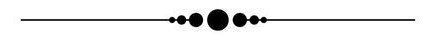
\includegraphics[scale=0.4]{end}
\end{figure}


\end{enumerate}
\end{document}